\documentclass[usenames,dvipsnames]{beamer}
\usepackage{../../shared/styles/mycommonstyle}

\title{Cross-Validation}
\date{\today}
\author{Nipun Batra and teaching staff}
\institute{IIT Gandhinagar}

\begin{document}
	\maketitle
	
	


\begin{frame}{Our General Training Flow}
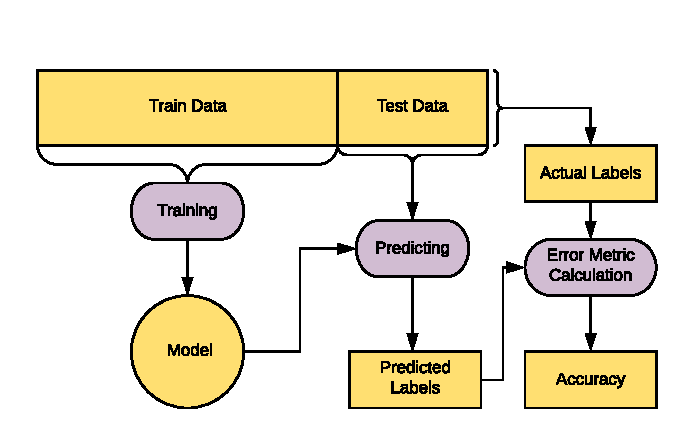
\includegraphics[width = 0.9\textwidth]{../assets/cross-validation/diagrams/general-workflow}
\begin{itemize}
	\item \pause Does not use the full dataset for training and does not test on the full dataset
	\item \pause No way to optimise hyperparameters
\end{itemize}
\end{frame}

\begin{frame}{How to use the full dataset for training?}
\begin{itemize}
	\item \pause Over multiple iterations, use different parts of the dataset for training and testing.
	\item \pause Typically done via different random splits of the dataset.
	\item \pause Challenge?
	\item \pause May not use every data point for training or testing
	\item \pause May be computationally expensive

\end{itemize}
	
\end{frame}

\begin{frame}{K-Fold cross-validation: Utilise full dataset for testing}
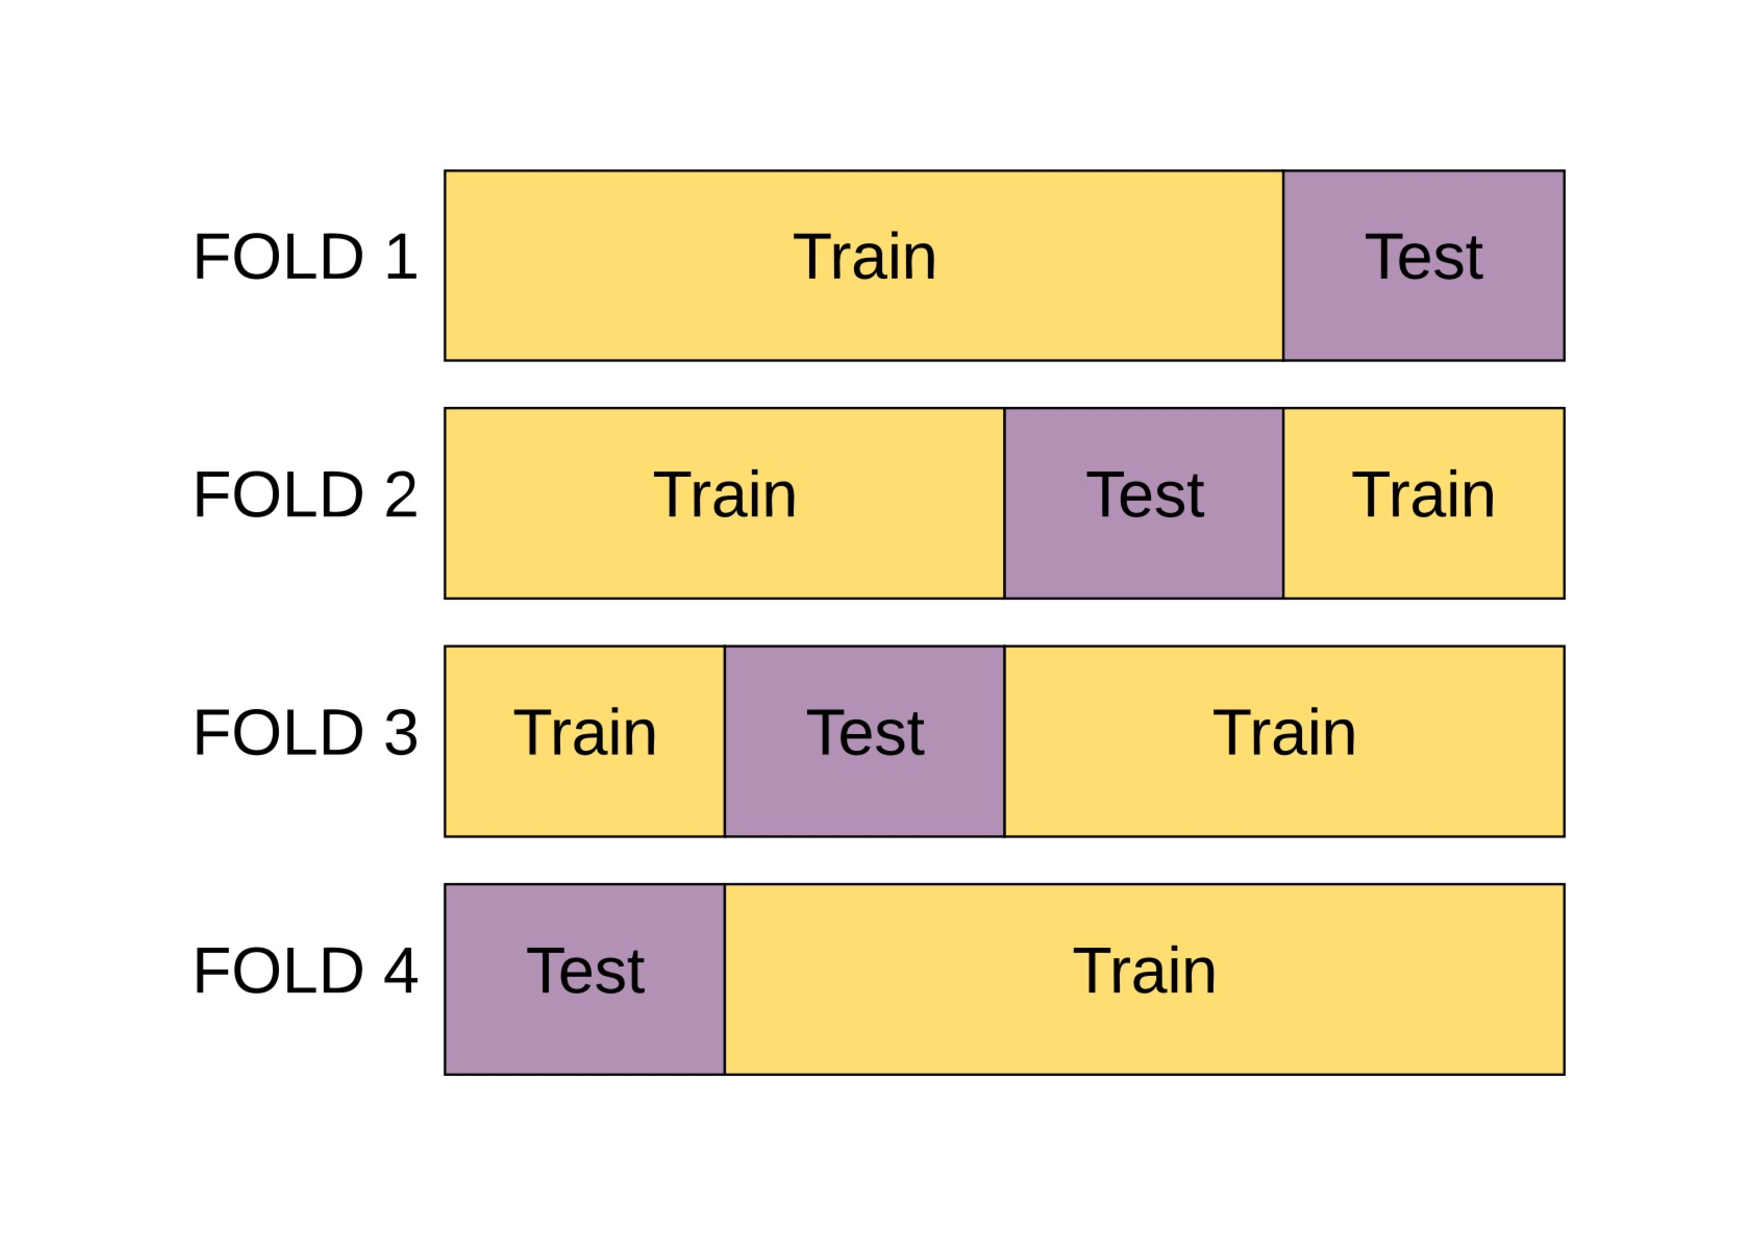
\includegraphics[width = \textwidth]{../assets/cross-validation/diagrams/cross-validation-train-test}
\pause Each data point is used for testing exactly once.
\end{frame}

\begin{frame}{Optimizing hyperparameters via the Validation Set}
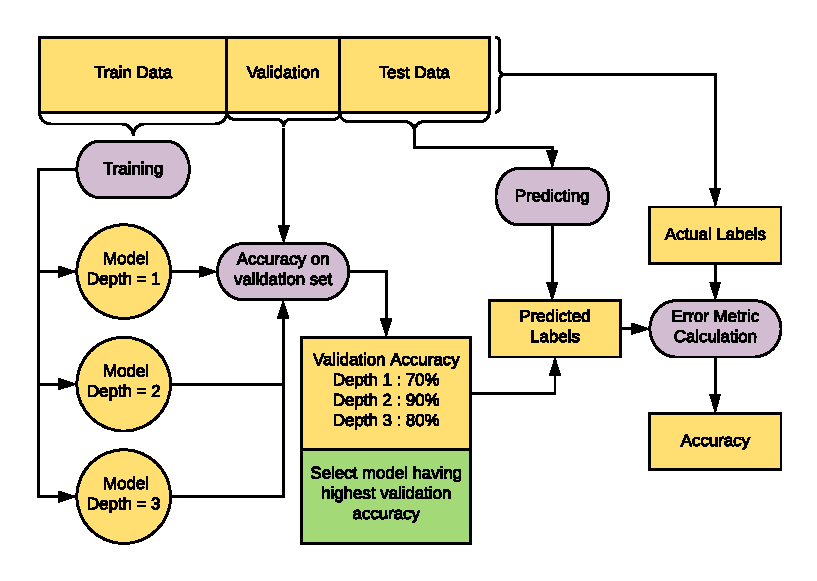
\includegraphics[width = \textwidth]{../assets/cross-validation/diagrams/validation-workflow}
\end{frame}

\begin{frame}{Nested Cross Validation}
Divide your training set into $K$ equal 	parts.\\
Cyclically use 1 part as ``validation set" and the rest for training.\\
Here $K = 4$
\begin{center}

\includegraphics[scale=0.7]{../assets/cross-validation/diagrams/cross-validation.pdf}
\end{center}
\end{frame}

\begin{frame}{Nested Cross Validation}
Average out the validation accuracy across all the folds\\
Use the model with highest validation accuracy\\
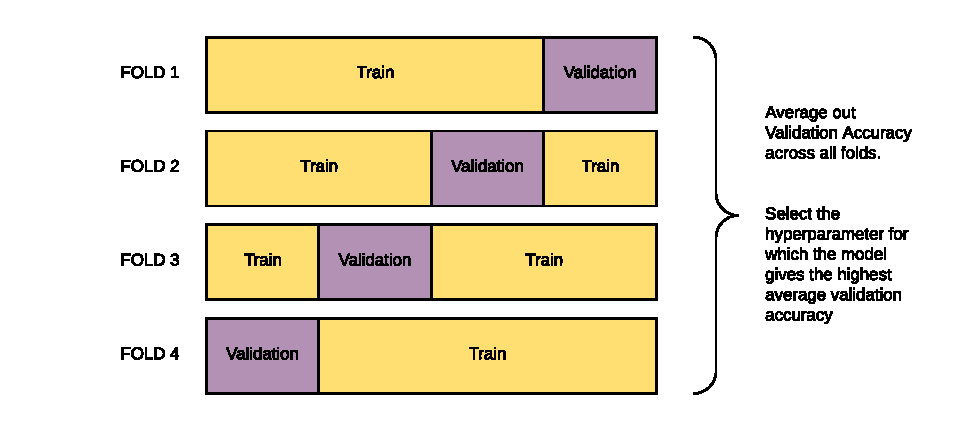
\includegraphics[width = \textwidth]{../assets/cross-validation/diagrams/cross-validation-avg.pdf}
\end{frame}

\begin{frame}{Next time: Ensemble Learning}
\begin{itemize}
\item How to combine various models?
\item Why to combine multiple models?
\item How can we reduce bias?
\item How can we reduce variance?
\end{itemize}
\end{frame}

\end{document}